 \subsubsection{UC10 - Gestione veicoli}
  \begin{figure}[H]
 	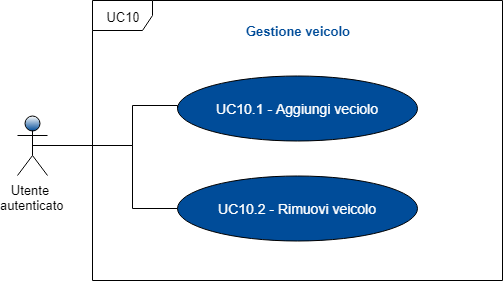
\includegraphics[width=9cm]{res/images/UC10Gestioneveicolo.png}
 	\centering
 	\caption{UC10 - Gestione Veicoli}
 \end{figure}
 \begin{itemize}
 	\item \textbf{Attori Primari}: utente autenticato;
 	\item \textbf{Descrizione}: l'utente visualizza i propri veicoli. Per ogni veicolo vengono visualizzate le seguenti informazioni:
 	\begin{itemize}
 		\item marca;
 		\item modello;
 		\item anno di immatricolazione;
 		\item rating;
 	\end{itemize}
 	\item \textbf{Precondizione}: l'utente accede al fragment\glosp per la gestione dei veicoli;
 	\item \textbf{Postcondizione}: l'utente visualizza le informazioni relative ai propri veicoli, con le eventuali operazioni disponibili su ognuno di essi.
 \end{itemize}
 \subsubsection{UC10.1 - Aggiunta veicolo}
 \begin{itemize}
 	\item \textbf{Attori Primari}: utente autenticato;
 	\item \textbf{Descrizione}: l'utente può aggiungere un mezzo di trasporto al proprio parco macchine;
 	\item \textbf{Scenario principale}: l'utente aggiunge un veicolo compilando gli appositi campi, ovvero:
 	\begin{itemize}
 		\item Inserimento marca veicolo [UC10.1.1];
 		\item Inserimento modello veicolo [UC10.1.2];
 		\item Inserimento anno d'immatricolazione veicolo [UC10.1.3].
 	\end{itemize}
 	e successivamente salverà il nuovo veicolo [UC10.1.4];
 	\item \textbf{Precondizione}: l'utente ha inserito correttamente tutti i campi necessari;
 	\item \textbf{Postcondizione}: il nuovo veicolo viene aggiunto ai veicoli posseduti.
 \end{itemize}
\begin{figure}[H]
	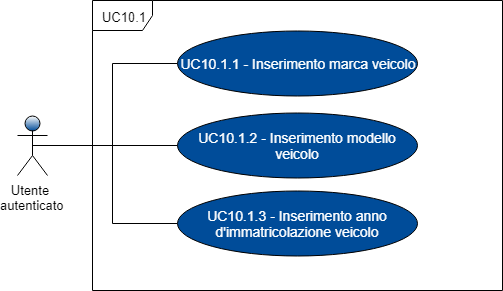
\includegraphics[width=9cm]{res/images/UC10-1Aggiungiveicolo.png}
	\centering
	\caption{UC10.1 - Aggiunta veicolo}
\end{figure}
\subsubsection{UC10.1.1 - Inserimento marca veicolo}
\begin{itemize}
	\item \textbf{Attori Primari}: utente autenticato;
	\item \textbf{Descrizione}: al fine di portare a termine il processo di inserimento di un nuovo veicolo l'utente deve inserirne la marca, campo ritenuto obbligatorio;
	\item \textbf{Scenario principale}: l'utente compila il campo relativo alla marca del veicolo;	
	\item \textbf{Precondizione}: l'applicazione ha reso disponibile il campo per l'inserimento della marca del veicolo;
	\item \textbf{Postcondizione}: l'utente ha compilato il campo con la marca.	
\end{itemize}

\subsubsection{UC10.1.2 - Inserimento modello veicolo}
\begin{itemize}
	\item \textbf{Attori Primari}: utente autenticato;
	\item \textbf{Descrizione}: al fine di portare a termine il processo di inserimento di un nuovo veicolo l'utente deve inserirne il modello, campo ritenuto obbligatorio;
	\item \textbf{Scenario principale}: l'utente compila il campo relativo alla marca del veicolo;	
	\item \textbf{Precondizione}: l'applicazione ha reso disponibile il campo per l'inserimento il modello del veicolo;
	\item \textbf{Postcondizione}: l'utente ha compilato il campo con il modello.	
\end{itemize}

\subsubsection{UC10.1.3 - Inserimento anno d'immatricolazione veicolo}
\begin{itemize}
	\item \textbf{Attori Primari}: utente autenticato;
	\item \textbf{Descrizione}: al fine di portare a termine il processo di inserimento di un nuovo veicolo l'utente deve inserirne l'anno di immatricolazione, campo ritenuto obbligatorio;
	\item \textbf{Scenario principale}: l'utente compila il campo relativo all'anno d'immatricolazione del veicolo;	
	\item \textbf{Precondizione}: l'applicazione ha reso disponibile il campo per l'inserimento dell'anno d'immatricolazione del veicolo;
	\item \textbf{Postcondizione}: l'utente ha compilato il campo con l'anno d'immatricolazione.	
\end{itemize}

\subsubsection{UC10.1.4 - Invio dati veicolo}
\begin{itemize}
	\item \textbf{Attori Primari}: utente autenticato;
	\item \textbf{Descrizione}: l'utente preme il pulsante per la conferma e l'invio dei dati del veicolo;
	\item \textbf{Scenario principale}: l'utente preme il pulsante di verifica ed invio dei dati;	
	\item \textbf{Precondizione}: i campi dati necessari per l'inserimento di un veicolo sono compilabili. È presente il pulsante per la conferma dei dati;
	\item \textbf{Postcondizione}: il nuovo veicolo viene inserito e l'utente potrà visualizzarlo nel proprio parco macchine.
\end{itemize}

\subsubsection{UC10.2 - Rimozione veicolo}
\begin{itemize}
	\item \textbf{Attori Primari}: utente autenticato;
	\item \textbf{Descrizione}: l'utente può rimuovere un mezzo di trasporto al proprio parco macchine;
	\item \textbf{Scenario principale}: l'utente può selezionare un veicolo e attraverso l'apposito pulsante rimuoverlo dal proprio parco macchine.
	\item \textbf{Precondizione}: l'applicazione mostra all'utente i propri veicoli e ne permette la selezione.
	\item \textbf{Postcondizione}: il veicolo selezionato viene rimosso dal parco macchine
\end{itemize}